\section{Effect of \nueCConepi sample on constraint strength}
\label{app:sample_comparison}

\Cref{sec:results} showed stronger than expected constraints from data for \deltacp, appearance and disappearance fits. To determine a potential explanation for this we chose to run an additional fit without the \nueCConepi sample, hereafter referred to as the 4-sample fit, with the fit using all samples being referred to as the 5-sample fit. It should be noted that the full 5-sample marginalisation toys were used for all fits, rather than using 4-sample marginalisation toys for the 4-sample fit. This means that the correlations among samples for the 4-sample fit are not handled correctly, but the effect from this is expected to be small.

\Cref{fig:sample_comparison} shows comparisons of the aforementioned fits for normal hierarchy. It can be seen that the constraint on the \deltacp and appearance fits is weakened in the absence of the \nueCConepi sample, while the disappearance contour is unaffected.

\begin{figure*}[htb]
	\center
	\begin{subfigure}[b]{0.49\textwidth}
		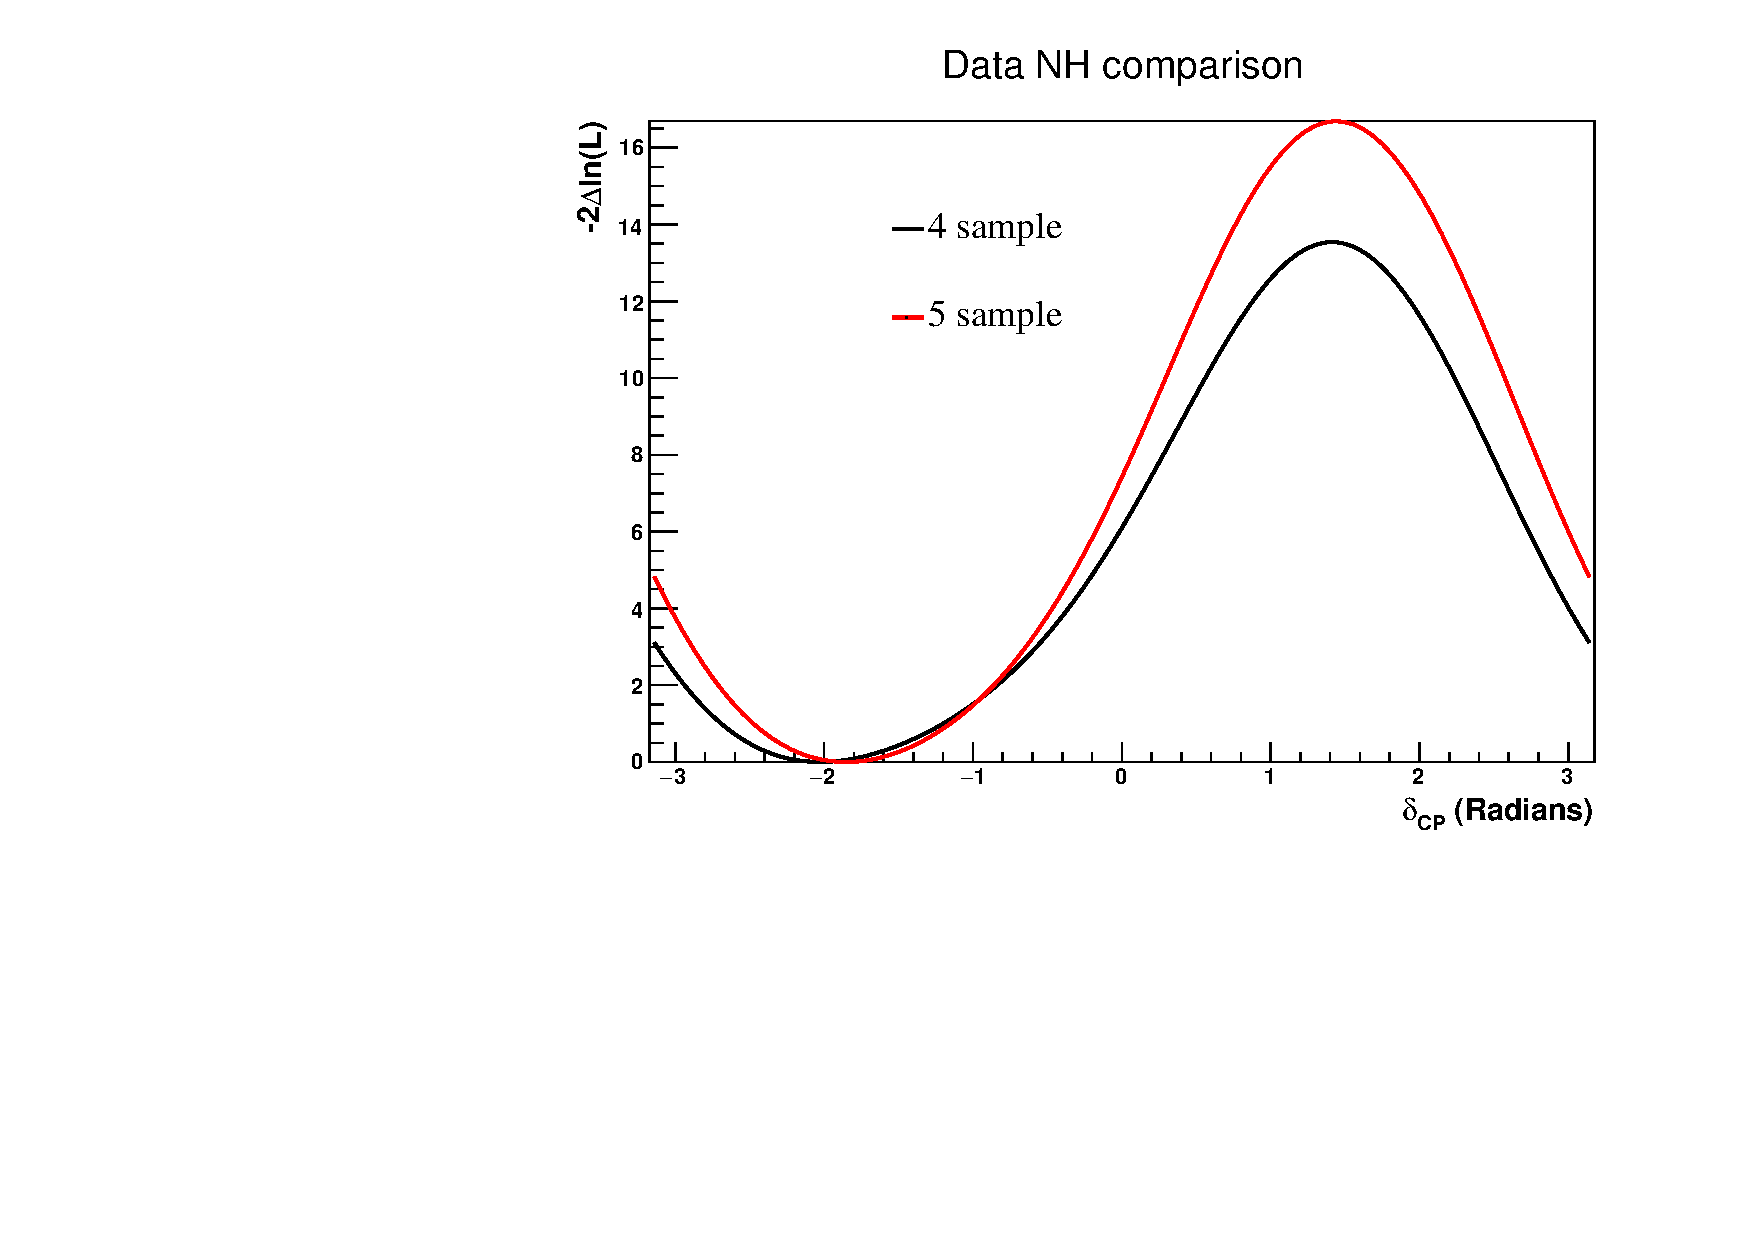
\includegraphics[width=0.9\textwidth]{data/sample_comparison/deltacp_nh_data_samples}
		\caption{\deltacp data fit}
	\end{subfigure}
	\begin{subfigure}[b]{0.49\textwidth}
		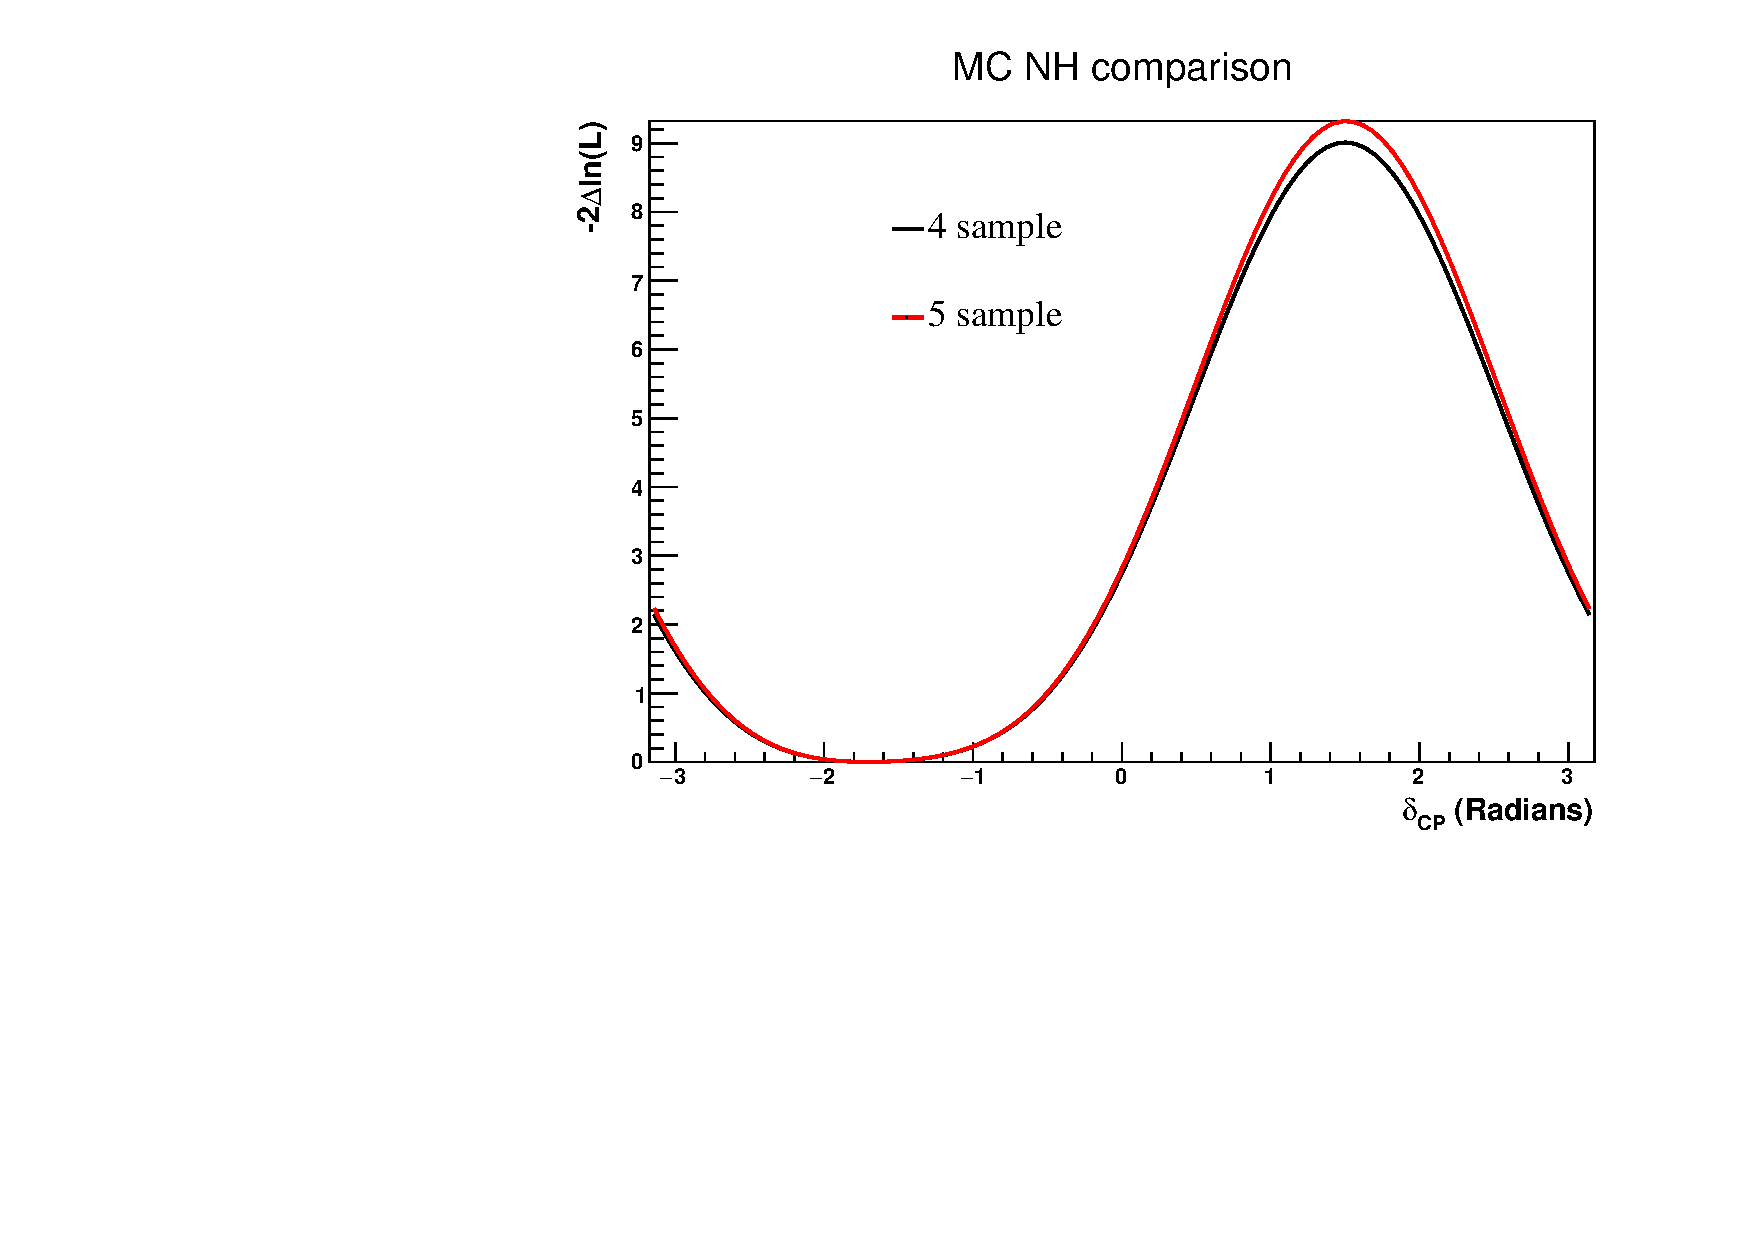
\includegraphics[width=0.9\textwidth]{data/sample_comparison/deltacp_nh_mc_samples}
		\caption{\deltacp MC fit}
	\end{subfigure}
	\begin{subfigure}[b]{0.49\textwidth}
		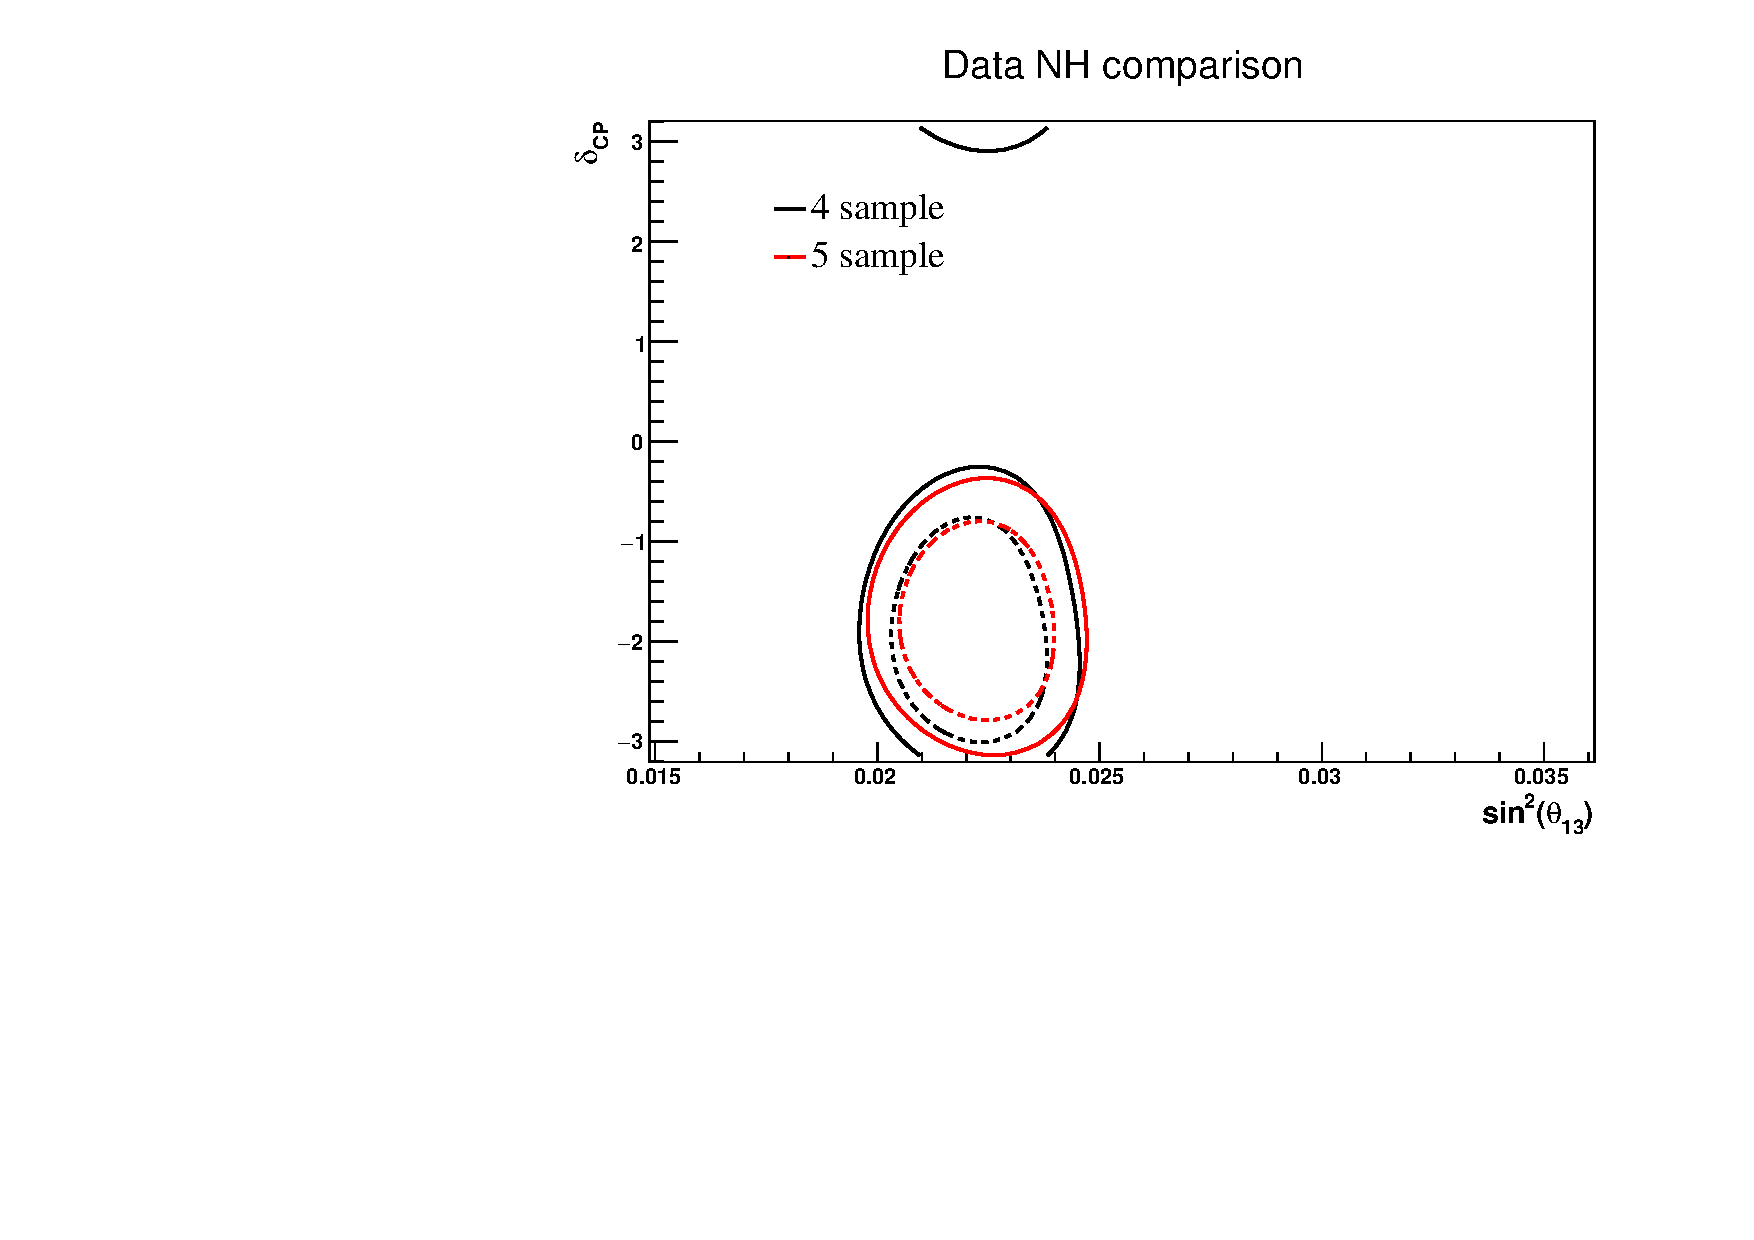
\includegraphics[width=0.9\textwidth]{data/sample_comparison/appearance_nh_data_samples}
		\caption{Appearance data fit}
	\end{subfigure}
	\begin{subfigure}[b]{0.49\textwidth}
		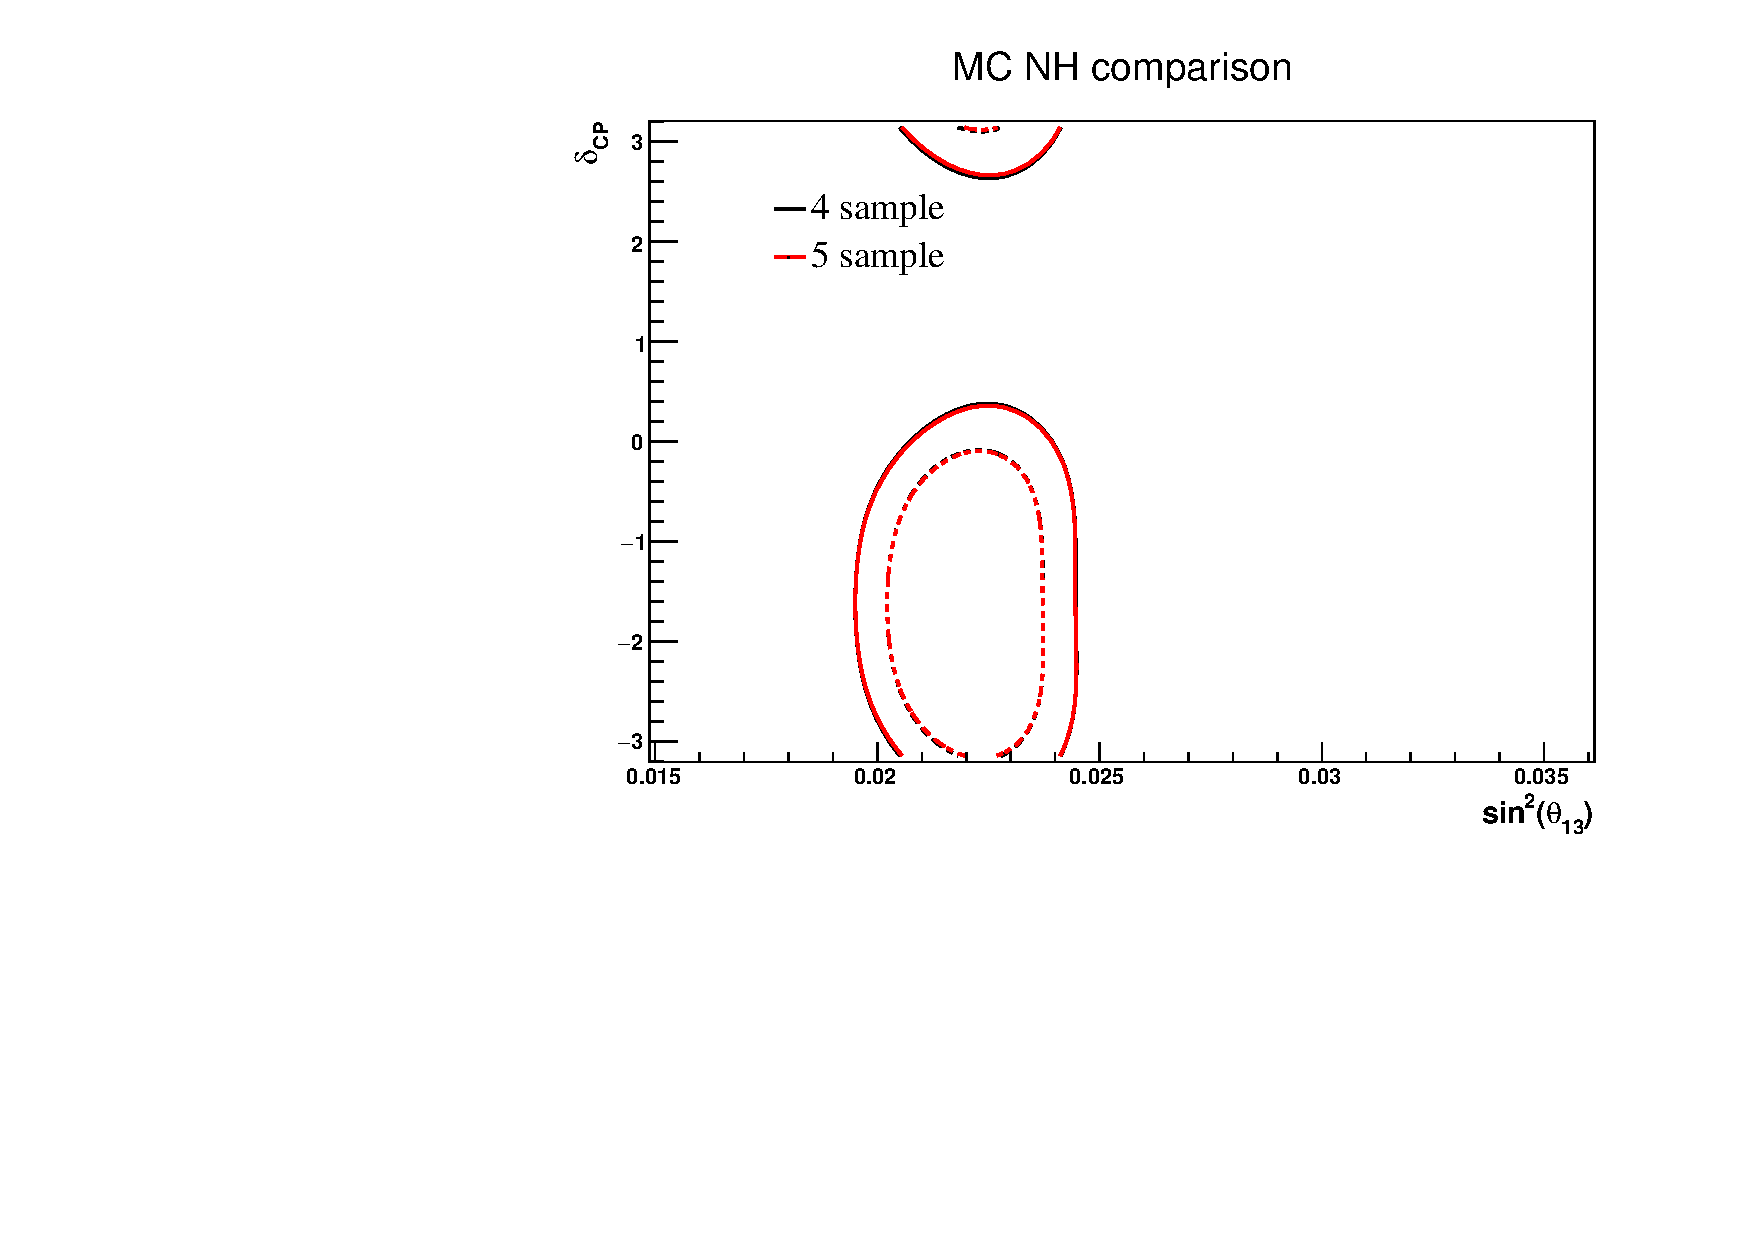
\includegraphics[width=0.9\textwidth]{data/sample_comparison/appearance_nh_mc_samples}
		\caption{Appearance MC fit}
	\end{subfigure}
	\begin{subfigure}[b]{0.49\textwidth}
		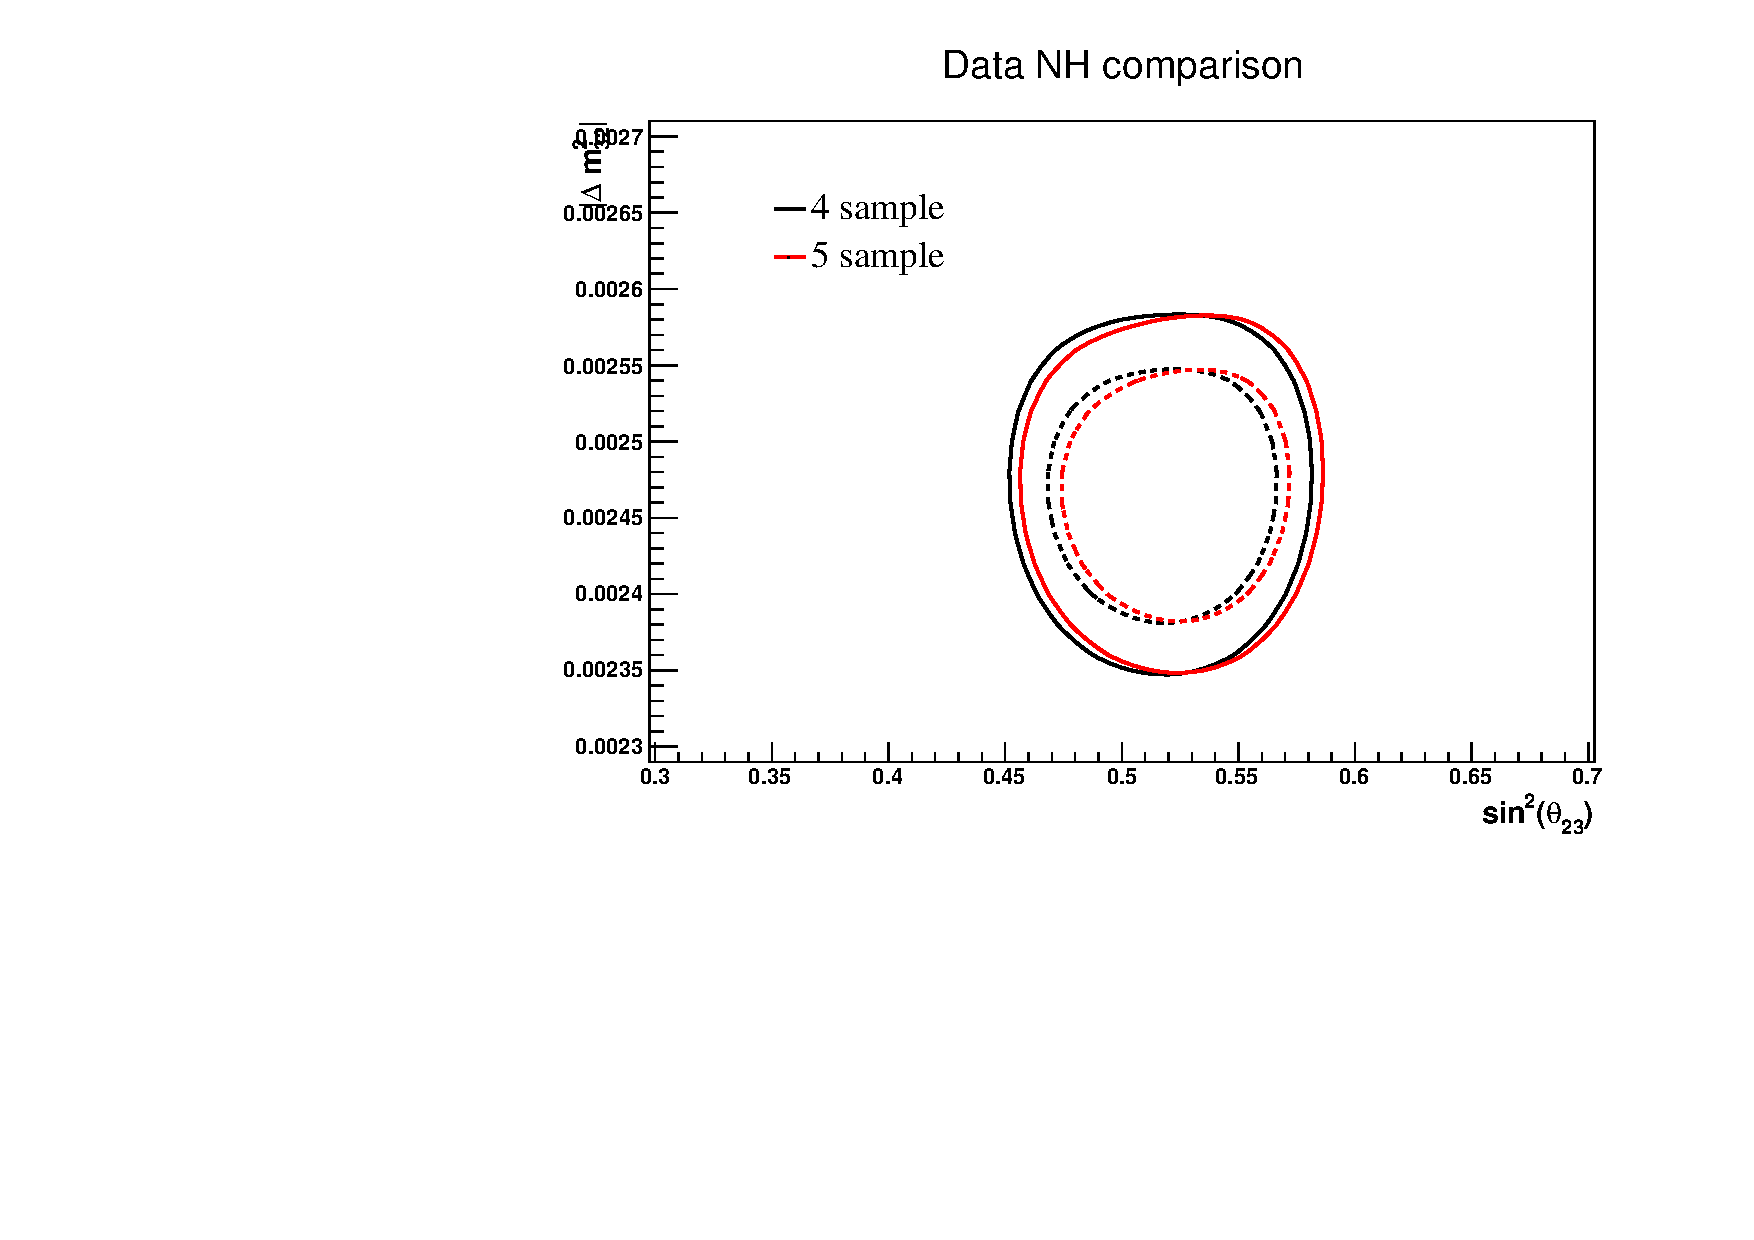
\includegraphics[width=0.9\textwidth]{data/sample_comparison/disappearance_nh_data_samples}
		\caption{Disappearance data fit}
	\end{subfigure}
	\begin{subfigure}[b]{0.49\textwidth}
		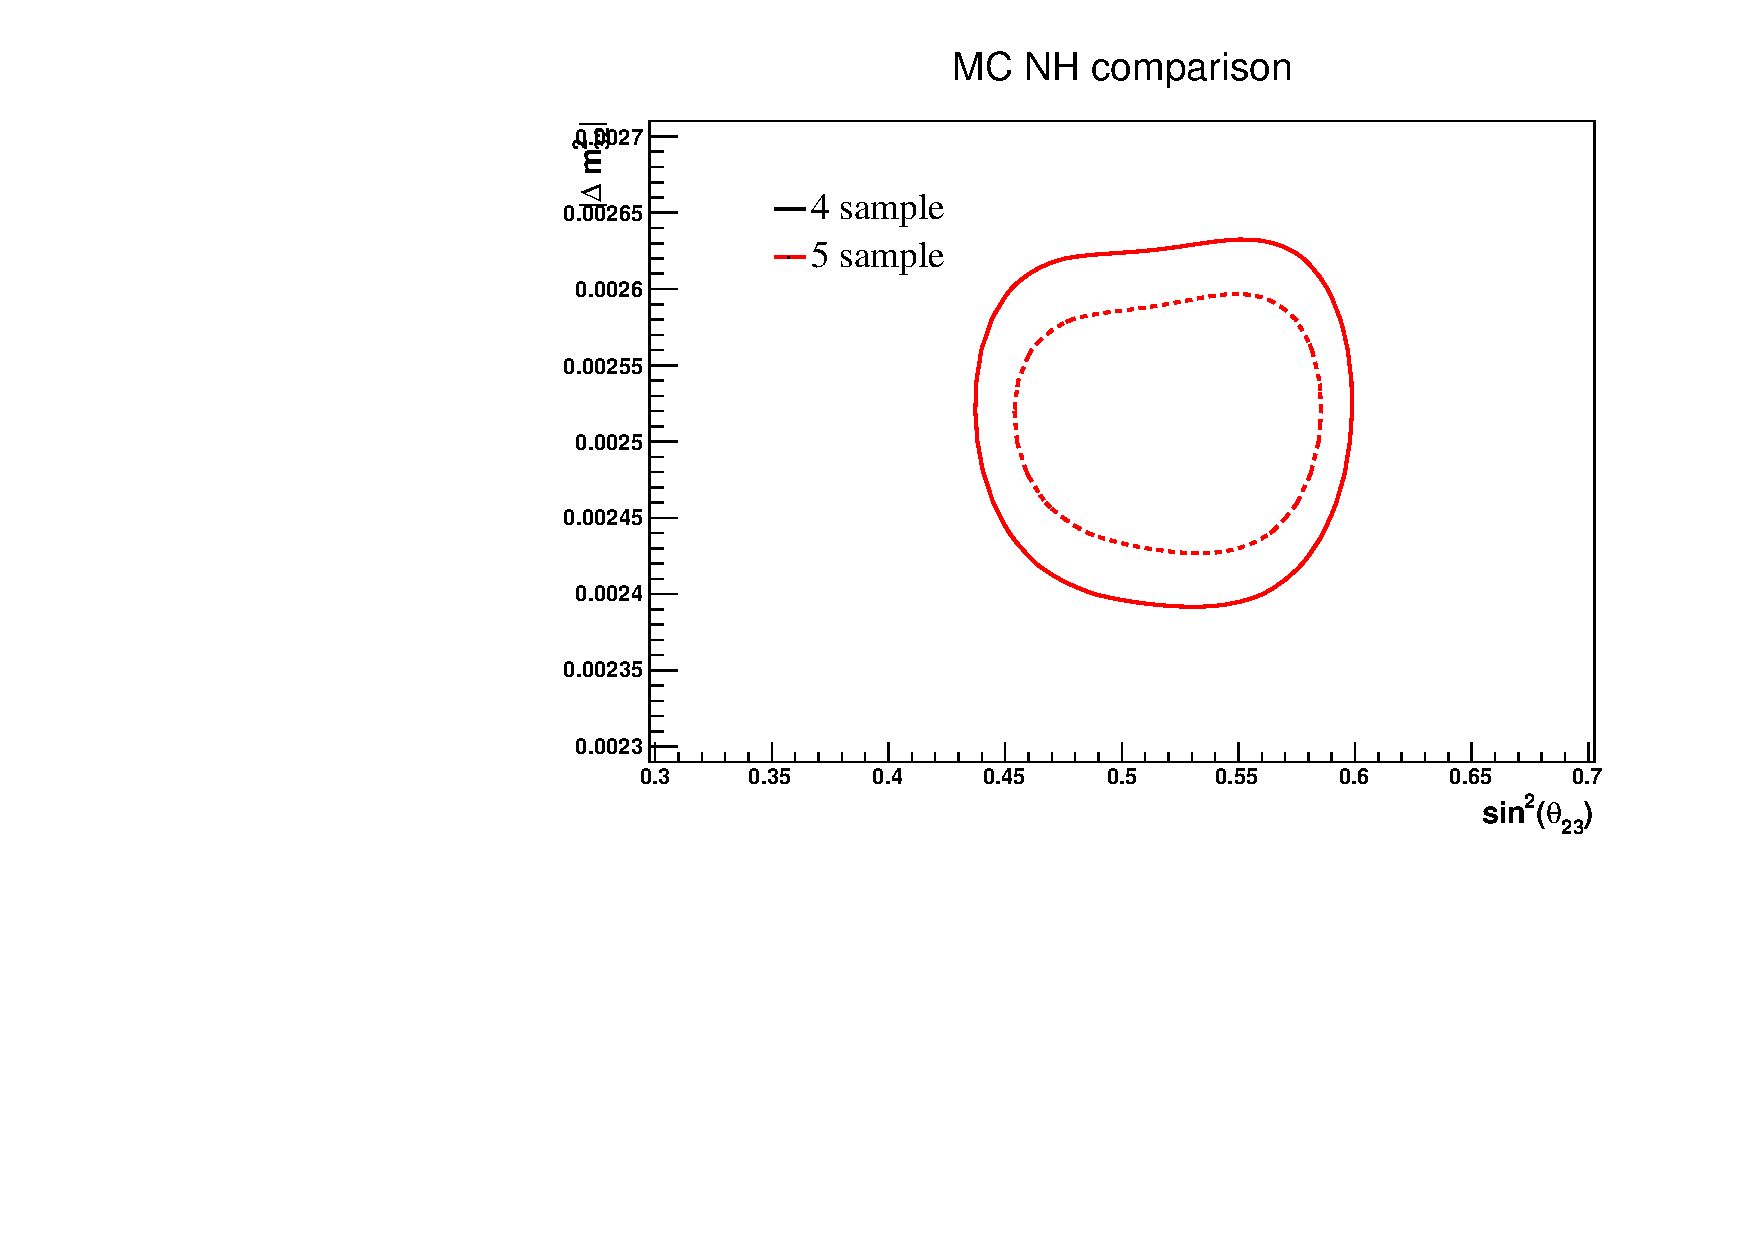
\includegraphics[width=0.9\textwidth]{data/sample_comparison/disappearance_nh_mc_samples}
		\caption{Disappearance MC fit}
	\end{subfigure}
	\caption {
		Fits of data and the Asimov A data set with four and five samples respectively.
	}
	\label{fig:sample_comparison}
\end{figure*}
\clearpage